\documentclass[oneside,12pt,a4paper]{book}	

% ---------------------------------------------------
% Preambulum
% ---------------------------------------------------

\usepackage[magyar,english]{babel}
\usepackage[utf8]{inputenc}
\usepackage{t1enc}
\usepackage{indentfirst}
\usepackage{graphicx}
\usepackage{amsmath}
\usepackage{amsfonts}
\usepackage{url}
\usepackage{algorithmic}
\usepackage{algorithm}
\usepackage{mdwlist}
\usepackage{listings}
\usepackage{wrapfig}
\usepackage{epigraph}
\usepackage{placeins}
\lstset{basicstyle=\footnotesize\ttfamily}
\newcommand{\inlinecode}{\texttt}
\DeclareGraphicsExtensions{.png,.jpg}
\usepackage[left=3.5cm,right=2.5cm,top=2.5cm,bottom=2.5cm]{geometry}
\linespread{1.3}

\usepackage{tikz}

\newcounter{treeline}

\newcommand{\treeroot}[1]{% Title
\node[above] at (0,0) {#1};%
\setcounter{treeline}{0}
}

\newcommand{\treeentry}[2]{% Title, Level
\draw[->] (#2-1,-\value{treeline}/2) -- (#2-1,-\value{treeline}/2-0.5) -- (#2+0.5,-\value{treeline}/2-0.5) node[right] {#1};
\stepcounter{treeline}
}

\newcommand{\altentry}[2]{% Title, Level
\draw[->] (#2-1,-\value{treeline}/2) -- (#2-1,-\value{treeline}/2-0.5) -- (#2+0.5,-\value{treeline}/2-0.5) node[right] {#1};
\foreach \x in {1,...,#2}
{   \draw (\x-1,-\value{treeline}/2) -- (\x-1,-\value{treeline}/2-0.5);
}
\stepcounter{treeline}
}

\DeclareMathOperator{\diag}{diag}
\setcounter{secnumdepth}{3}
\setcounter{tocdepth}{3}

\begin{document}
\clearpage
\thispagestyle{empty}
\hspace{-10pt}\begin{tabular}{p{3cm} p{1cm} p{10cm}}
\raisebox{-2.5cm}{
\includegraphics[scale=0.2]{ELTE_logo}} & &
\large{\foreignlanguage{magyar}{Eötvös Loránd Tudományegyetem\newline Informatikai Kar\newline
 Programozási Nyelvek és \newline Fordítóprogramok Tanszék}}
\end{tabular}
\vspace{0.4cm}
\hrule
\vspace{6cm}
\begin{center}
\LARGE{\textbf{Applying slicing algorithms on large code bases}}
\end{center}
\vspace{3cm}
\begin{tabular}{p{7cm} p{8cm}}
\large{Tibor Brunner \vspace{5pt} \newline doktorandusz} &
\large{\foreignlanguage{magyar}{ Olivér Hechtl \vspace{5pt} \newline programtervező informatikus MSc}}
\end{tabular}\vspace{6cm}
\begin{center}
\large{Budapest, 2017}
\end{center}
\newpage
\setcounter{page}{1}
\pagenumbering{arabic}
\pagestyle{plain}
\tableofcontents

\chapter{Introduction}
\epigraph{Everyone knows that debugging is twice as hard as writing a program in the first place. So if you're as clever as you can be when you write it, how will you ever debug it?}{\textit{Brian Kernighan}}

Nowadays, there are a lot of tools available for debugging. A developer can examine call stacks, variable informations, and so on. There are a lot of times when a bug is when some variable does not behave like the writer of that code part would expect. When the programmer discovers it, he must follow back the path of assignments, and find out where did it get an unexpected value. Program slicing targets this kind of debugging. We can define a program slice as a part of the program which contains a selected statement, and all other statements which influences it, or gets influenced by it. These two types are respectively called backward and forward slicing. Basically this is what many programmers do intuitively, when facing with bugs. In this thesis, I'll introduce a few approaches for computing slices, and describe a working prototype tool application, which can analyze C++ programs, and compute slices of them. I've used the help of the Clang/LLVM compiler infrastructure, which builds the AST of the program and provides an interface to analyse it using C++.

%TODO describe the structure of the thesis.
In the second chapter, I will describe three known algorithms and analyze them by performance, effectiveness and usability regarding slicing. In the next chapter, I will introduce the Clang/LLVM compiler infrastructure, and it's library for analyzing C++ code, and how I used it for the task. In the last chapter, I will describe the algorithm I have used to implement slicing, and how I implemented it.

\chapter{Slicing, methods and efficiency}
\section{About slicing}
For better understanding programs, programmers organize code into structures. They write sub-problems into functions, and organize variables and data to structs. Also, with object oriented design, they combine the related functions and variables into classes which define objects. These are all good for separating the data, and the procedures on data. But these are not helpful when we need to examine a flow of data in the program. Slicing gets useful in this scenario. This is a program analysis technique introduced by Mark Weiser\cite{weiser84}. In his paper, he wrote: ``Program slicing is a decomposition based on data flow and control flow analysis''. We define slicing as a subset of the program, which only includes the statements which may influence the value regarding the selected statement, or may get influenced by that value, depending on the direction of interest. In other words, slicing filters the statements of the program, and include only those which have transitive control or data dependency regarding the selected statement. 

\section{Types of slicing}
There is two different type of slicing known: static and dynamic. While dynamic slicing gets the statements which could affect the selected statement at a particular execution of the program with a fixed input, static slicing examines it statically, including all possible statements which could affect that selected statement. In this thesis, I'll focus on static slicing methods. There are two different subtypes of static slicing, backward and forward. They are indicating the relevant statements' direction from our selected statement. 

\section{Methods for slicing}
We can construct slices via various methods on different representations of the program. All of these are using some kind of graph structures, which can be traversed through for searching the transitive data dependences.

\subsection{Dependences}
Before I describe the various methods currently available for slicing, we must get to know what dependences in programs are. There are two kinds of dependences: control and data. They can be defined by the control flow graph (CFG) of the program. Given the following example:
\begin{figure}[h]
\begin{lstlisting}[language=C++]
int main(){
  int sum = 0;
  int i = sum;
  while (i < 11){
    sum += i;
    i++;
  }
}
\end{lstlisting}
\caption{Example program}
\label{fig:example_prog}
\end{figure}

\begin{wrapfigure}{r}{0.4\textwidth}
  \centering
    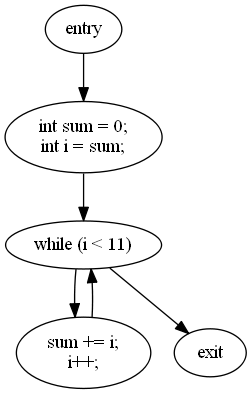
\includegraphics[width=0.38\textwidth]{horwitz_cfg.png}
  \caption{Control-flow graph}
  \label{fig:horwitz_cfg}
\end{wrapfigure}

It's control-flow graph can be seen on \ref{fig:horwitz_cfg}. This type of graph is created from the program by grouping the statements into basic blocks. Each basic block consists a maximal amount of consecutive statements without any jumps. In a high-level language, such as C++, a jump can be either a branch statement, like an \texttt{if} and a \texttt{switch-case}, or a loop statement, like a \texttt{while}. In the example, we can see that it's CFG consists three basic blocks, and two special blocks, namely \texttt{entry} and \texttt{exit}, which represent the entry and exit points of the program, respectively.

Therefore, control dependence can be defined in the knowing of post-dominance. As written in \cite{slicing-survey}:

"A node \textit{i} in the CFG is \textit{post-dominated} by a node by \textit{j} if all paths from \textit{i} to STOP pass through \textit{j}. A node \textit{j} is \textit{control dependent} on a node \textit{i} if (i) there exists a path \textit{P} from \textit{i} to \textit{j} such that \textit{j} post-dominates every node in \textit{P}, excluding \textit{i} and \textit{j}, and (ii) is not post-dominated by \textit{j}."

It basically means that every statement under a branch or loop are control dependent of the control statement's predicate. Excluding the unstructured and structured jump statements, \texttt{continue},\texttt{break} and \texttt{goto}, drawing control dependences between statements creates a tree, with the root being the inspected function, and control statements form the branches. I discuss later in detail in the implementation chapter the control dependences created by structured jumps. 

A data dependence between two statements means that if we change their order, the meaning of the program changes, or becomes ill-formed. There are two types of data dependences: \textit{flow dependences} and \textit{def-order dependences}. According to Horwitz\cite{horwitz-interproc}, we can define these with the following rules:

There is a flow dependence between statement $s_1$ and $s_2$ if:
\begin{enumerate}
  \item $s_1$ defines variable $x$.
  \item $s_2$ uses $x$.
  \item There is a path between $s_1$ and $s_2$ in program execution with no intervening definitions of $x$ in between, and $s_2$ can be reached by control from $s_1$. 
\end{enumerate}

Definition in this context means a bit different than usual: it can be either an initial definition of a variable, or an assignment where $x$ is on the left side. In compiler theory, flow-dependence referred as reaching definition of a variable.

In the presence of loops, there are two further classifications of flow-dependence: loop-carried and loop-independent. A flow-dependence is loop-carried if it satisfies all rules above and also:
\begin{enumerate}
  \item includes a backedge to the predicate of the loop and
  \item $s_1$ and $s_2$ are both enclosed in the loop.
\end{enumerate}

Backedge means that there is a flow dependence between the statement and the predicate of the loop, therefore the loop uses the variable which that statement defines. In the example above, the loop is dependent on the the statement \texttt{i++}, so from \texttt{i++} there is a backedge to the \texttt{while} loop.

Loop-independent flow-dependences has no backedge to the loop predicate. They are drawn on the statements used in the body of the loop which does not change on every loop iteration. There can be both type of dependences to the same statement. 

On the other hand, def-order dependence between statement $s_1$ and $s_2$ is different from loop-independent flow-dependences only in that $s_2$ instead of using $x$, it also defines it. The other two rules stays the same. 

These definitions are used in all slicing methods, but differently. I will elaborate these in each section.

\subsection{Data flow equations}
\subsubsection{The algorithm}
This method is created by Mark Weiser. It is based on the analysis of the CFG. As he wrote in \cite{weiser84}, he defines a slice regarding a \textit{slicing criterion}, which consists of a pair $(n, V)$ where $n$ is a statement of the program and $V$ is a subset of the program's variables, which we are slicing on. He also wrote that a slice of a program is an executable, which has only the relevant statements in it.

To calculate which statements should be included in the slice, he defines two sets of variables: \textit{directly} and \textit{indirectly relevant} variables. As written in \cite{slicing-survey}, he provides the following equations for them:

For determining \textit{directly} relevant variables and statements:

For each edge $i \rightarrow_{CFG} j$ in the CFG:
\begin{align*}
R^0_C(i) &= R^0_C(i) \cup \{ v | v \in R^0_C(j), v \notin \textsc{Def}(i) \} \cup \{ v | v \in \textsc{Ref}(i), \textsc{Def}(i) \cap R^0_C(j) \neq \emptyset \} \\
S^0_C &= \{ i | (\textsc{Def}(i) \cap R^0_C(j) \neq \emptyset, i \rightarrow_{CFG} j \}
\end{align*}

And for determining \textit{indirectly} relevant variables and statements:
\begin{align*}
B^k_C &= \{ b | \exists i \in S^k_C, i \in \textsc{Infl}(b) \} \\
R^{k+1}_C(i) &= R^k_C(i) \cup \bigcup_{b \in B^k_C} R^0_{(b, \textsc{Ref}(b))} (i) \ \\
S^{k+1}_C &= B^k_C \cup \{ \textsc{Def}(i) \cap R^{k+1}_C(j) \neq \emptyset, i \rightarrow_{CFG} j \} 
\end{align*}

He also says that a slice is statement-minimal if it couldn't have less statements. The slice then is computed in two steps:
First by determining \textit{directly} relevant variables by the equation above. In it, $\textsc{Def}(i)$ and $\textsc{Ref}(i)$ means the variables that statement $i$ defines or uses (references), respectively. $R^0_C(i)$ will contain the directly relevant variables of statement $i$. We take the following base values: in the slicing criterion: $R^0_C(n) = V$ and for all other sets initialized as $\emptyset$. As it can be seen from the first equation above, to get the $R^0_C$ value for a node, it must use the computed values from every direct node following it in the CFG. Weiser states in his work[1], that this algorithm is a simplification of the usual data flow information extraction, which would use a PRE set to represent preservation of variable values. Reading the first equation, we see that variable $v$ is in the $R^0_C(i)$ set either if:
\begin{enumerate}
\item $v$ is in the slicing criterion $V$,
\item or $v$ is in \textsc{Ref}(i) and the $R^0_C$ set of any of the following CFG node $j$ has a value which is also in \textsc{Def}(i) 
\item or $v$ is not in \textsc{Def}(i) but $v$ is in $R^0_C(j)$.
\end{enumerate}
The last constraint ensures the propagation of the `may be used` variables through statements which does not use nor reference the variables in the slicing criterion. 

The second equation $S^0_C$ then contains the statements which are included in the slice. It goes through the CFG from start and collects all variables that may have an influence on the slicing criterion. I've listed the sets of variables which are in \textsc{Def}, \textsc{Ref} and $R^0_C$ of the statements of the example program above in the table below.

\begin{table}[h]
  \centering
  	\begin{tabular}{|l|l|l|l|l|}
\hline
No. & Statement                & \textsc{Def} & \textsc{Ref}   & $R^0_C$      \\ \hline
1   & \texttt{int sum = 0;}    & \texttt{sum} & $\emptyset$    & $\emptyset$  \\ \hline
2   & \texttt{int i = sum;}    & \texttt{i}   & \texttt{sum}   & \texttt{sum} \\ \hline
3   & \texttt{while (i < 11)}  & $\emptyset$  & \texttt{i}     & \texttt{i}   \\ \hline
4   & \texttt{sum += i;}       & \texttt{sum} & \texttt{sum,i} & \texttt{i}   \\ \hline
5   & \texttt{i++}             & \texttt{i}   & \texttt{i}     & \texttt{i}   \\ \hline
  \end{tabular}
  \caption{Results of the algorithm for the given example and criterion \texttt{(i++,\{i\})} }
  \label{tab:weiserExampleTable}
\end{table}

In this case, the set $S^0_C$ contains statements no. 1, 2, and 5. As we see, this slice is incomplete since it does not include the \texttt{while} statement. For this to be included, further iterations should be done. In the equations above, Weiser introduces the \textsc{Infl} set for every statement $i$, which consists all statements which are control dependent on $i$. In our example, it is the empty set for all statements except the \texttt{while}, which consists statements no. 4 and 5. Using this, he defines the $B^k_C$ set, which includes all statements which have a statement in it's \textsc{Infl} set which is included in $S^k_C$.

Now using $B^k_C$, we can add the \texttt{while} statement since the slicing criterion is control dependent on it. This is defined in the last equation, which is almost the same as the second, but it also includes the $B^k_C$ set in it. When facing with nested branch, or looping statements, multiple levels of indirect dependences must be considered. The $R^{i+1}_C$ set contains these for each level. Because of this, Weiser's algorithm needs iterations for achieving the correct slice. With every iteration $k$, $R^k_C$ and $S^k_C$ sets are creating a series of non-decreasing sets by size, and they reach a fixpoint which are called $R_C$ and $S_C$, respectively. The final $S_C$ set contains the slice for the criterion.

I must note that this method computes the whole slice for any criterion, and can only be used for forward and/or backward slicing if the algorithm gets prepared, partial CFG graphs of the program to analyze.

\subsubsection{Efficiency}
Weiser states that the complexity for computing $S_C$ is $O(n\ e\ log\ e)$. He notes that this slice is not always the smallest, since it could include statements which cannot influence the slicing variable. He shows it in the following example program:
\begin{lstlisting}
a = constant
while(p(k)){
  if (q(c)){
    b = a;
    x = 1;
  }else{
  	c = b;
  	y = 2;
  }
  k++;
}
z = x + y;
write(z)
\end{lstlisting}

For criterion \texttt{C = (write(z),\{z\})}, the set $S_C$ will contain the first statement, but it does not have an influence on \texttt{z} since on any path by which \texttt{a} can influence \texttt{c} will execute \texttt{x = 1} and \texttt{y = 2}, therefore \texttt{z} becomes a constant value in this case. 

However, computing slices with Weiser's algorithm needs little information from the program, since it requires only the CFG and the \textsc{Ref} and \textsc{Def} sets for every statement.
The downside is that it only computes whole slices, and since the criterion is fixed, it needs to compute every set in the equations if we need a slice for a different slicing criterion of the program.

\subsection{Information flow relations}
\subsubsection{The algorithm}
This algorithm is created by Bergeretti and Carré\cite{information-flow}. It has a different approach than Weiser's: it associates the program's statements with relations: that which expression may affect which variable. These relations has the definitions in the table below.
\clearpage
\begin{table}[t]
  \centering
  	\begin{tabular}{l}
Empty statements                                                                            \\
$D_S = \emptyset$                                                                           \\
$\lambda_S = \emptyset$                                                                     \\
$\rho_S = \iota$                                                                            \\
$P_S = V$                                                                                   \\
$\mu_S = \emptyset$                                                                         \\
\hline                                                                                      
Assignment Statements, in a form of \texttt{v = e}                                          \\
$D_S = \{v\}$                                                                               \\
$\lambda_S = \Gamma(e) \times \{e\}$                                                        \\
$\rho_S = \Gamma(e) \times \{v\} \cup (\iota - \{(v,v)\})$                                   \\
$P_S = V - \{v\}$                                                                           \\
$\mu_S = \{(e,v)\}$                                                                         \\
\hline                                                                                      
Sequences of statements, in a form of A;B                                                   \\
$D_S = D_A \cup D_B$                                                                        \\
$\lambda_S = \lambda_A \cup \rho_A\lambda_B$                                                \\
$\rho_S = \rho_A\rho_B$                                                                     \\
$P_S = P_A \cap P_B$                                                                        \\
$\mu_S = \mu_A\rho_B \cup \mu_B$                                                            \\
\hline                                                                                      
Conditional statements, in a form: \texttt{if (\textit{e}) A else B}                        \\
$D_S = D_A \cup D_B$                                                                        \\
$\lambda_S = (\Gamma(e) \times \{e\}) \cup \lambda_A \cup \lambda_B$                        \\
$\rho_S = (\Gamma(e) \times (D_A \cup D_B)) \cup \rho_A \cup \rho_B$                        \\
$P_S = P_A \cup P_B$                                                                        \\
$\mu_S = (\{e\} \times (D_A \cup D_B)) \cup \mu_A \cup \mu_B$                               \\
\hline                                                                                      
Conditional statements, without else: \texttt{if (\textit{e}) A}                            \\
$D_S = D_A$                                                                                 \\
$\lambda_S = (\Gamma(e) \times \{e\}) \cup \lambda_A$                                       \\
$\rho_S = (\Gamma(e) \times D_A) \cup \rho_A \cup \iota$                                    \\
$P_S = V$                                                                                   \\
$\mu_S = (\{e\} \times D_A) \cup \mu_A$                                                     \\
\hline                                                                                      
Repetitive statements, in a form: \texttt{while (\textit{e}) A}                             \\
$D_S = D_A$                                                                                 \\
$\lambda_S = \rho^*_A((\Gamma(e) \times \{e\}) \cup \lambda_A)$                   \\
$\rho_S = \rho^*_A((\Gamma(e) \times D_A) \cup \iota)$                            \\
$P_S = V$                                                                                   \\
$\mu_S = (\{e\} \times D_A) \cup \mu_A\rho^*_A((\Gamma(e) \times D_A) \cup \iota)$\\
  \end{tabular}
  \caption{Table of information flow relations}
  \label{tab:informationFlowTable}
\end{table}
\FloatBarrier
The statements are classified into two primitive types: Empty and Assignment, and three hiearchical types: Sequence, Conditional with \texttt{else} branch, without \texttt{else} and the Repetitive statements. They are constructed from the control-flow graph. For analysis, they define \textit{variables} and \textit{expressions}. For Assignment, it's left side is the variable, and it's right side is the expression associated with it. Only this type of statement has a variable. For Conditional and Repetitive statements their conditional expression used, and Empty and Sequence has no variable or expression. There's also the definition of $\Gamma(e)$ which consists the variables which appear in $e$. We define $E$ and $V$ which contains all of the variables and expressions of the program. In $D_S$ there are the variables which $S$ \textit{may define}. In $P_S$ are the variables which $S$ \textit{may preserve}. The `multiplication` sign which we do not write between relations is the \textit{relational composition}:
For relations $X$ and $Y$, where $X \subseteq A \times B$ and $Y \subseteq B \times C$:
\begin{equation}
XY = \{(a,d) \in A \times C | (a,b) \in X, (c,d) \in Y, b = c\}
\end{equation}

The main three binary relations are the following:
\begin{enumerate}
\item $\lambda_S$, from $V$ to $E$
\item $\mu_S$, from $E$ to $V$
\item $\rho_S$, from $V$ to $V$
\end{enumerate}

For a statement $S$, $v \in V, e \in E: v \lambda_S e$ means that `the value of $v$ on entry to $S$ \textit{may be used} in the evaluation of the expression $e$ in $S$.' Taken the following program:
\begin{lstlisting}[language=C++]
void fn(int x){
  read(n);             //1
  int i = 1;           //2
  while (i <= n){      //3
    if (i \% 2 = 0) {  //4
      x = 17;          //5
    }
    else{              
      x = 18;          //6
    }
    i = i + 1;         //7
  }
  write(x);            //8
}
\end{lstlisting}

It can be seen that in case of the \texttt{while} statement, variable $n$ and the predicate of \texttt{while} is in the $\lambda_{\texttt{while}}$ relation.

Taking a look at $\mu_S$, it means that for expression $e$ and variable $v$ : $e \mu_S v$ `a value of e in $S$ \textit{may be used} in obtaining the value of the variable $v$ on exit from $S$'. Looking at our example again, for the expression of \texttt{if} statement and variable $x$, $\mu_{\texttt{if}}$ holds, since the execution of assignments to $x$ are control dependent on the \texttt{if} statement.

It is basically the dual relation of $\lambda_S$, which will be very useful in aspect of slicing.

The final relation $\rho_S$ can be constructed from $\lambda_S$,$\mu_S$ and $P_S$:
\begin{equation}
\rho_S = \lambda_S\mu_S \cup \Pi_S,\  where \ \Pi_S = \{(v,v) \in V \times V\ |\ v \in P_S\}.
\end{equation}

This combination of $\lambda_S$ and $\mu_S$ creates a relation which is for $v,w \in V$:
\begin{enumerate}
\item either the entry value of $v$ to $S$ \textit{may be used} obtaining the exit value of $w$, or
\item $v = w$, and $S$ \textit{may preserve} $v$.
\end{enumerate}

In the code above, for the \texttt{if} statement we get the \texttt{\{(i,x),(i,i),(n,n),(x,x)\}} set of pairs for it's $\rho_{\texttt{if}}$ relation, since it can be seen that variable $i$ is in the predicate, so it may be used for evaluating $x$, but also, if the predicate does not hold, then the statement preserves all three variables of the program. 

These relations are different for each type of statements.

For Empty, the sets $D_S$, $\lambda_S$ and $\mu_S$ are the empty set since it has no variable in it. $P_S$ is the whole $V$ because it does not modify any variable, therefore it preserves every variable. Also, for the $\rho_S$ relation we define the identity relation $\iota$ for variables $v \in V$:
\begin{equation}
\iota = \{(v,w) \in V \times V | v = w\}.
\end{equation}
Which means the same as the $P_S$ set.

For Assignment statements, the definitions are simple. They have the form of \texttt{v = e}, so in $D_S$, there's $v$, in $P_S$, there's every variable minus $v$, since the statement assigns the value of the expression $e$ to it. In case of $\lambda_S$, it is trivial that the variables of $e$ - denoted by $\Gamma(e)$ - may be used in evaluating $e$. Also, $\mu_S$ defines that the right-hand side effects the left-hand side of the assignment. As written above, $\rho_S$ can be expressed as:
\begin{equation}
\begin{split}
\rho_S &= \lambda_S\mu_S\ \cup\ \Pi_S\ =\ (\Gamma(e) \times {e})({(e,v)})\ \cup\ \Pi_S\ =\\
&= (\Gamma(e) \times {v})\ \cup\ \Pi_S\ =\ (\Gamma(e) \times {v})\ \cup\ (\iota\ -\ \{(v,v\})
\end{split}
\end{equation}

In Assignment, $\Pi_S$ does not contain the variable, because it is being changed.

In the case of Sequence of statements, they have no direct variable or expression associated with them. They represent the single arrow between two nodes in the CFG. So, for the sequence of statements $A;B$, the relation $e \lambda_S v$ contains either
\begin{enumerate}
\item $e$ which is in $A$ and $v \lambda_A e$ or
\item $e$ is in $B$ and there is a variable $w$ that $v \rho_A w$ and $w \lambda_B e$.
\end{enumerate}

As defined above, $\rho_A$ gets all the variables from statement $A$ which are preserved or may be used, therefore they are fitting in the definition for the sequence.

Similarly, $\mu_S$ contains pairs of $(v,e)$ which either
\begin{enumerate}
\item $e$ is in $A$ and there is a variable $w$ that $e \mu_A w$ and $w \rho_B v$ or
\item $e$ is in $B$ and $e \mu_B v$
\end{enumerate}

The duality of $\lambda_S$ and $\mu_S$ can again be seen.
For $\rho_S$, we can substitute the formulas:
\begin{equation}
\begin{split}
\rho_S\ &=\ (\lambda_A\ \cup\ \rho_A\lambda_B)(\lambda_A\ \cup\ \rho_A\lambda_B)\ \cup\ (\Pi_A\ \cap\ \Pi_B)
\end{split}
\end{equation}

For brevity, I don't follow through the substitution here. The result of it is $\rho_A\rho_B$. 
In case of a sequence of statements which has more than two statements in it, we can define it by nesting: $(((A;B);C);...)$. The ordering of parentheses are irrelevant.

For Conditional statements, there is a control dependence between it's predicate $e$ and the statements $A,B$ in them. Therefore,
$(v,e)$ is in $\lambda_S$ if
\begin{enumerate}
\item $e$ is the predicate and $v \in \Gamma(e)$
\item $e$ is in $A$ and $v \lambda_A e$ or
\item $e$ is in $B$ and $v \lambda_B e$.
\end{enumerate}
%todo more text

In case of $\mu_S$, $(v,e)$ is in the relation if:
\begin{enumerate}
\item $e$ is the predicate, and either $A$ or $B$ define $v$, or
\item $e$ is in $A$ and $e \mu_A v$ or
\item $e$ is in $B$ and $e \mu_B v$.
\end{enumerate}

With substituting $\lambda_S$ and $\mu_S$ into the formula of $\rho_S$ above, we get:
\begin{equation}
\rho_S = (\Gamma(e) \times (D_A \cup D_B)) \cup \rho_A \cup \rho_B
\end{equation}

When the Conditional statement has no \texttt{else} branch, we can substitute it with an Empty expression, gaining the simplified formulas which can be seen in table \ref{tab:informationFlowTable}.

Bergeretti in his paper states that Repetitive statements can be expressed as an infinite sequence of nested conditional  statements in a form of:
\begin{lstlisting}
if(e){
  A;
  if(e){
    A;
    ...
  }
}
\end{lstlisting}

Therefore we can get the formula of $\lambda_{\textsc{Rep}}$ if we repeatedly use $\lambda_{\textsc{Cond}}$ and $\lambda_{\textsc{Seq}}$, gaining the following:
\begin{equation}
\lambda_S = \rho^*_A((\Gamma(e) \times \{e\}) \cup \lambda_A)
\end{equation}
where $\rho^*_A$ is the \textit{transitive closure} of $\rho_A$.

For any relation $R$, it's transitive closure is the fixpoint of the following set:
\begin{equation}
R^* = \bigcup_{i \in \{1,2,...\}} R^i
\end{equation}
The other two relations can be similarly derived by applying their Conditional and Sequence versions, thus getting:
\begin{equation}
\begin{split}
\rho_S &= \rho^*_A((\Gamma(e) \times D_A) \cup \iota) \\
\mu_S &= (\{e\} \times D_A) \cup \mu_A\rho^*_A((\Gamma(e) \times D_A) \cup \iota)
\end{split}
\end{equation}

For determining a slice of a program with these relations, Bergeretti describes the definition of partial statements, with the formula:
\begin{equation}
E^v_S = \{e \in E\ |\ e \mu_S v\}
\end{equation}

As it can be seen from the definition of $\mu_S$, this results in the whole slice for variable $v$, if the given statement $S$ is the `statement' of the whole program, as a Sequence of top-level statements. It also gets the \textit{expressions} which may affect the variable, and not the statements consisting it. However, using $\mu_S$, we can create formulas which effectively get the desired statements from the program. It can be seen that with the dual nature of $\mu_S$ and $\lambda_S$, they can be used for backward and for forward slicing, respectively. 

\subsubsection{Efficiency}

This algorithm is throroughly defines the flow of data across statements, taking control dependences into account. Further extensions, like applications for \texttt{switch-case} expressions can be added by defining the relations for them, on the basis of the current ones. It needs deeper examination of the source code than Weiser's method, for getting all the variables of the expressions, and statements. However, if we parse the program code, and collect the $D_S$, $v$, $e$, and $\Gamma(e)$ sets, and the variables and expressions for each statement, we can compute many different slices for different variables and statements for the program. In the case of large codebases, this is an important aspect of the algorithm. 

In the presence of loops, calculating the reflexive closure takes additional time. Bergeretti states the following for the complexity of the calculation of relations: $\rho_S$ has a worst case asymptotic $O(|V|^3)$. Therefore, for all statements it is $O(|E| \times |V|^3)$. For $\lambda_S$ and $\mu_S$, it is $O(|E| \times |V|^2)$ for each statement, or $O(|E|^2 \times |V|^2)$. 
If we compare these with Weiser's, it is clear that this algorithm requires more computation for slicing the program for the first time, however Bergeretti noted that these times are not problematic in real life examples.



\subsection{Dependence graph based slicing}
\subsubsection{The algorithm}
The third algorithm is first written by Ottenstein and Ottenstein\cite{ottenstein}, and has been a base for different slicing techniques, used by Susan Horwitz\cite{horwitz-interproc}, and \cite{use-of-slicing-horwitz}, \cite{program-analysis-via-graph-reachability-reps}, \cite{slicing-with-jumps} and \cite{slicing-oop}.  

This algorithm uses the Program Dependence Graph, which is a directed graph constructed either from the control-flow graph or the abstract syntax tree \textit{(AST)} of the program. Horwitz describes this graph thoroughly in her paper\cite{horwitz-interproc}. It contains the control dependence and data dependence subgraphs. The nodes of it are the statements of the program. There is a special node called the entry node, which is considered to be before any statement in the CFG. Building the graph is done in two steps: first by creating the control dependence subgraph, then drawing the data dependence edges in it. Control dependence edges has boolean labels: they are either \texttt{true} or \texttt{false}.

There is a control dependence edge between two nodes $v_1$ and $v_2$ if:
\begin{enumerate}
\item $v_1$ is the entry node, and $v_2$ is a statement which is not under any loop or branch.
\item $v_1$ is a loop or branch statement, and $v_2$ is \textit{immediately} nested under $v_1$. If $v_1$ is a loop statement, then the label of the edge is \texttt{true}, if it is a branch statement, then if $v_2$ is under the `then` branch, the label is \texttt{true}, and \texttt{false} otherwise.
\end{enumerate}

The control dependence subgraph has similar structure as the AST. It is the direct consequence of that the loop and branch statements has other statements nested in them. In \cite{efficient-pdg}, there are region nodes created for predicate of each loop or branch. In practice, I have found these unnecessary to deal with. I will later discuss it in the chapter about the implementation. 

After constructing the control dependence subgraph, data dependence edges are added. The meaning of this kind of edge between $v_1$ and $v_2$ is that if we change the order of these statements then the program may become ill-formed or the computation is changed. In the aspect of slicing, there are two main different type of edges: \textit{flow dependence} and \textit{def-order dependence}. In compiler theory, in data-flow analysis there is the `use-def' or `def-use' chain, which has similar definitions what Horwitz describes in her paper. There is a flow dependence edge between nodes $v_1$ and $v_2$ if:
\begin{enumerate}
\item $v_1$ is a node which defines variable $x$ and
\item $v_2$ uses $x$ and
\item Control can reach $v_2$ after $v_1$ in an execution path which does not contain any intervening definition of $x$.
\end{enumerate}

The third rule is easy to verify if the PDG is built using the CFG, but using the `def-use' chains, it also can be derived from the AST. 

In the case of loops, there are two further sub-types of flow dependence edges: \textit{loop-carried} and \textit{loop-independent}. In addition to the three rules above, Loop-carried edges must hold that:
\begin{enumerate}
\item The path in the third rule contains a backedge to the predicate of loop $L$ and
\item $v_1$ and $v_2$ are both part of loop $L$.
\end{enumerate}

Loop-independent edges are not keeping the first rule above, so the path does not contain a backedge to the predicate.
There is a def-order dependence edge between node $v_1$ and $v_2$ if:
\begin{enumerate}
\item $v_1$ and $v_2$ defines the same variable and
\item There is a execution path between $v_1$ and $v_2$ without any intervening definition of that variable.
\end{enumerate}
\clearpage
Taken the following example program:
\begin{figure}[h]
\lstset{numbers=left}
\begin{lstlisting}[language=C++]
int main(){
  int x = 0;
  int y = 1;
  while(x >= 0){
    if (x > 0){
      y = x; //2. use here
    }else{
      x = 3;
    }
    x = 2; //1. define here
  }
}
\end{lstlisting}
\caption{Example for loop-carried dependences}
\label{fig:example_prog_3}
\end{figure}

\begin{wrapfigure}{r}{0.5\textwidth}
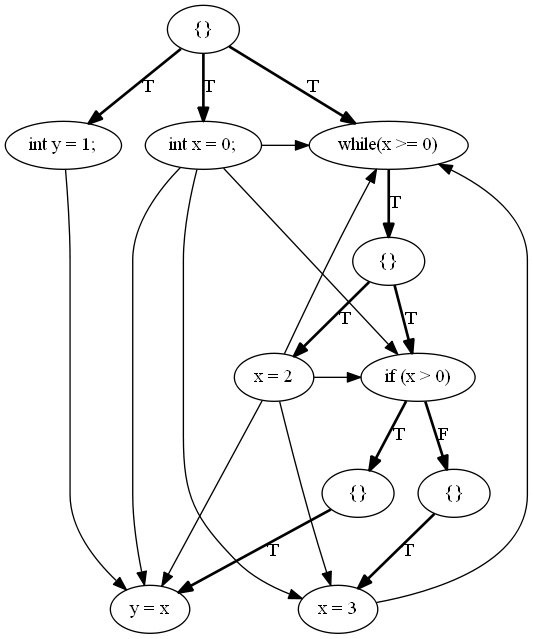
\includegraphics[width=0.5\textwidth]{loop_carried_test}
\caption{PDG of \ref{fig:example_prog_3}}
\label{fig:example_prog_3_PDG}
\end{wrapfigure}
We can see the created PDG of it on figure \ref{fig:example_prog_3_PDG}. The bold arrows represent the control dependence edges and the others are the data dependence edges. In her paper, Horwitz creates loop edges to the statements which are under a loop, but regarding slicing, they are not making a difference. As it can be seen, the nodes labeled \texttt{\{\}} are the brackets which consist multiple statements. I have created this example to show how a loop-carried edge can be found between different scopes under a loop statement. The comments in the example code shows the order of `def-use' relationship created by the loop: when control reaches $1.$, $x$ gets defined, then in the second iteration control goes into the true branch of the \texttt{if} statement and reaches $2.$, creating a `def-use' data dependence between the two statements. Among this, there are examples of def-order dependence edges: between line 8. and line 10., and also between the initial definition of $x$ and other definitions later. 

Covering every case which could occur in a source code, drawing data dependence edges are a non-trivial task. I will explain the details in the implementation chapter. However, the PDG itself when built, is a very useful abstraction of the program. To slice regarding a statement and variable in the program, we need to do only a graph reachability search in the graph over the control and data dependence edges. 

If we store the edges of the graph bidirectionally, the difference becomes only the direction of search between creating backward and forward slices. To show how a result of it looks, I have created an example of a backward slice on \ref{fig:example_prog_3_backward_slice}, regarding the $x$ variable on line 9.
\begin{figure}[h]
\centering
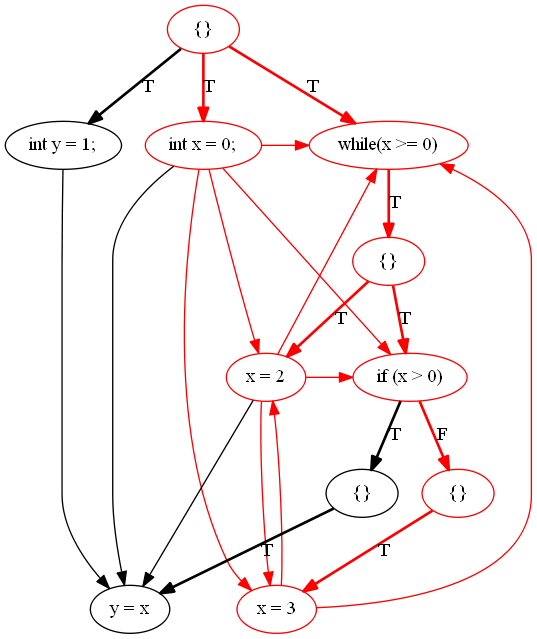
\includegraphics[width=0.7\textwidth]{loop_carried_test_backward_slice}
\caption{Backward slice of \ref{fig:example_prog_3}}
\label{fig:example_prog_3_backward_slice}
\end{figure}


% todo write more


\chapter{LLVM/Clang infrastructure}
\section{About Clang}

LLVM is a compiler infrastucture which is created mainly for program optimization during compile, link and runtime. It is written in C++ and language-agnostic itself, and uses an intermediate representation (LLVM IR) of the programs created in numerous languages. LLVM stands for \textbf{Low Level Virtual Machine} which was the initial target for the project, but since then it has grown to a massive infrastructure for program compilation and toolchains. LLVM does not handle the parsing and syntactic error checking in the languages, and separates this part via the IR. It was initially developed for C and C++, but since then there are numerous language frontends for a wide variety of languages including Haskell, Ada, Ruby, Python, etc. 

Clang is a compiler frontend for C,C++ and Objective-C, using LLVM as a backend for code generation. Clang is also written in C++, and has a library-based architecture which allows the compiler for not just compiling, but to build useful tools with it. For example, QtCreator IDE - an Integrated Development Environment - can use Clang as a `code model', for syntactically and semantically check the code in the editor, making error correcting much easier for the developer. There are also numerous tools built on the Clang using it as a library for parsing C++ code, for gaining information of it or performing source-to-source transformations. The Clang Static Analyzer is one of the most well-known tool of them, which is designed for analyzing and pointing flaws and possible runtime errors in a source code, statically, so without running it. It can detect possible division by zeroes, array overindexing, nullpointer dereferences, and so on. The prototype tool of this thesis uses similar techniques to achieve efficient program analysis, which will be discussed later in detail.

\section{The Clang AST}

The internal representation of C++ source code in Clang is using the \textbf{Abstract Syntax Tree} (AST\cite{Clang-AST}). Since it is written in C++, it uses the language's object-oriented features for encoding the structure of the program into a large class hiearchy, keeping all relevant information of a language element in an AST node.

Taken the example from Chapter 2:
\begin{lstlisting}[language=C++]
int main(){
  int sum = 0;
  int i = sum;
  while (i < 11){
    sum = sum + i;
    i++;
  }
}
\end{lstlisting}
\begin{figure}[h]
\lstset{
xleftmargin=-80pt,
aboveskip=\smallskipamount,
belowskip=\smallskipamount}
\begin{lstlisting}
FunctionDecl 0x595bd10 <horwitz.cc:1:1, line:8:1> line:1:5 main 'int (void)'
`-CompoundStmt 0x2716a50 <col:11, line:8:1>
  |-DeclStmt 0x2716868 <line:2:3, col:14>
  | `-VarDecl 0x2716810 <col:3, col:13> col:7 used sum 'int' cinit
  |   `-IntegerLiteral 0x2716848 <col:13> 'int' 0
  |-DeclStmt 0x27168e8 <line:3:3, col:14>
  | `-VarDecl 0x2716888 <col:3, col:11> col:7 used i 'int' cinit
  |   `-ImplicitCastExpr 0x27168d8 <col:11> 'int' <LValueToRValue>
  |     `-DeclRefExpr 0x27168c0 <col:11> 'int' lvalue Var 0x2716810 'sum' 'int'
  `-WhileStmt 0x2716a38 <line:4:3, line:7:3>
    |-<<<NULL>>>
    |-BinaryOperator 0x2716940 <line:4:10, col:14> '_Bool' '<'
    | |-ImplicitCastExpr 0x2716930 <col:10> 'int' <LValueToRValue>
    | | `-DeclRefExpr 0x27168f8 <col:10> 'int' lvalue Var 0x2716888 'i' 'int'
    | `-IntegerLiteral 0x2716910 <col:14> 'int' 11
    `-CompoundStmt 0x2716a20 <col:17, line:7:3>
      |-BinaryOperator 0x27169d8 <line:5:5, col:17> 'int' lvalue '='
      | |-DeclRefExpr 0x2716958 <col:5> 'int' lvalue Var 0x2716810 'sum' 'int'
      | `-BinaryOperator 0x27169c0 <col:11, col:17> 'int' '+'
      |   |-ImplicitCastExpr 0x27169a0 <col:11> 'int' <LValueToRValue>
      |   | `-DeclRefExpr 0x2716970 <col:11> 'int' lvalue Var 0x2716810 'sum' 'int'
      |   `-ImplicitCastExpr 0x27169b0 <col:17> 'int' <LValueToRValue>
      |     `-DeclRefExpr 0x2716988 <col:17> 'int' lvalue Var 0x2716888 'i' 'int'
      `-UnaryOperator 0x2716a08 <line:6:5, col:6> 'int' postfix '++'
        `-DeclRefExpr 0x27169f0 <col:5> 'int' lvalue Var 0x2716888 'i' 'int'
\end{lstlisting}
\caption{Clang AST of the example}
\label{fig:clang_ast}
\end{figure}

Clang enables us to dump it's AST via a compiler option, which can be seen on figure \ref{fig:clang_ast}.

The type of the nodes has a class hierarchy which has no common ancestor. There are a several base types, but only two are important for implementing slicing algorithms: the \texttt{Decl} and \texttt{Stmt} class. As it is logical, they encode a generic declaration, and statement, respectively. For example in the AST above, \texttt{FunctionDecl}, \texttt{VarDecl} are Decls, and \texttt{WhileStmt}, \texttt{CompoundStmt} and \texttt{DeclStmt} are Stmts. Also, it can be seen that Stmts create a clean tree hierarchy, where a predicate of a while loop belongs under it, enabling the AST to describe complex expressions. There is an API created for accessing the nodes' properties, which supports iterators on their children with \texttt{begin()} and \texttt{end()} much like the C++ standard library. For variable declarations, there is a wrapping \texttt{DeclStmt}, and for every block of code denoted by curly braces, there is a \texttt{CompoundStmt} associated with it. 

The Clang AST has a bit different logic in naming language elements than we would expect. It encodes assignments in a more generic \texttt{BinaryOperator}, and the API provides the \texttt{IsAssignment()} boolean method for it. It also encodes a defined variable's access in a \texttt{DeclRefExpr}, and if they are used on a right-hand side of an operator, it uses implicit cast expressions for casting them from lvalue to rvalue.

The source positions are also encoded in the nodes, but for space efficiency, they only store offsets. To access the correct visible position of them, we need to ask the \texttt{SourceManager} class, which can get the exact location of a node. 

\subsection{The RecursiveASTVisitor class}

Clang provides the \texttt{LibTooling} library to work with the AST. First, Clang parses the source code, and performs the compilation steps necessary to build the AST for us. Therefore if there's an error in the code, we won't get a partial AST. After then, we must provide a few classes which then can take care to run our action as a compilation step. The entry point is the \texttt{ASTFrontendAction} class, which creates an \texttt{ASTConsumer}, which can access the AST of the whole translation unit. Clang provides the \texttt{RecursiveASTVisitor} class, where we can create two types of methods for processing nodes: \texttt{Visit<NodeType>} and \texttt{Traverse<NodeType>}, where we put the node type which we want to process in the name of the method. With Visit, we can access the node, but Traverse can be used for controlling the traversal of the nodes, for example, if we do not want to visit any node under an If Statement, or to swap the traversal order of the two branches.

I have started the implementation with this API, but soon found out about the AST Matchers, which provided a better and easier to use solution.

\section{AST Matchers}

Although the RecursiveASTVisitor class could be enough for processing the AST, it could get easily complicated and require a lot of repeated code, making the tool less maintainable. However, there is a very useful API included with LibTooling of Clang, the ASTMatchers. With them, we can define the nodes we look for in the AST in a chain of matcher calls, which is a small domain-specific language defined for this specific task, but written in C++, naturally. For example, the following expression:
\begin{lstlisting}
binaryOperator(isAssignmentOp(),
    hasLHS(ignoringImpCasts(declRefExpr(to(varDecl().bind("lval"))))),
    anyOf(
      hasRHS(forEachDescendant(
      	expr(declRefExpr(to(varDecl().bind("rval")))))),
      hasRHS(anything())
    )).bind("binop");
\end{lstlisting}

Has a \texttt{binaryOperator} matcher, so with the internal boolean predication \\ \texttt{isAssignmentOp}, we can specify that it should match on assignment operators only. Via \texttt{hasLHS} and \texttt{hasRHS} inner matchers, we can specify what should be on the left and right side of the matched operator. And finally, the \texttt{anyOf} matcher can take arbitrary amount of arguments - which are also matchers - and becomes true if any of it's matchers are true. 

This only specifies what nodes we want to work with. For processing them, there is the \texttt{bind()} method, where we can specify a string identifier for the matched node. In the example above, there is a match for every assign statement, and every variable in them, separately. Every matcher has a callback function which is called every time when a node matching our specified matcher matches. We can define the processing method for the matches, and extract the statements or declarations bound via \texttt{bind} in it. The example shows how can we extract the variable declarations referenced in the \texttt{DeclRefExprs} in the assignment.

These ASTMatchers have a lot of similarities in common for querying with an NoSQL database query language. The separation of matching and processing enables us to avoid writing a lot of `boilerplate' code, and provides an intuitive way of specifying the desired information to query from the AST.

There are three types of matchers:
\begin{enumerate}
\item Node: match a specific type of AST node,
\item Narrowing: match attributes on AST nodes,
\item Traversal: allow traversal between AST nodes.
\end{enumerate}

In the previous section, in RecursiveASTVisitor, Visit was the equivalent of the Node matchers here. Every match expression starts with a node matcher, and they take arbitrary amount of parameters and match if all parameters returns true. There are a node matcher for every type of node in the AST. They are the ones which support the \texttt{bind} method. 

Narrowing matchers are boolean expressions which are narrowing down the set of nodes of the current type to match on. For example, \texttt{isAssignmentOp} is one of them, which can be used in \texttt{BinaryOperator} matchers. There are a few special logical matcher of this kind (\texttt{allOf}, \texttt{anyOf}, \texttt{anything}, \texttt{unless}), which can be used to build more complex matchers, as it can be seen from the example that with \texttt{anyOf} we specify that the right-hand side of the BinaryOperator has either a variable or something else, with \texttt{anything}. 

The Traversal matchers are different from the Traverse method from RecursiveASTVisitor. They can be used to specify the child or subexpression of the node we want to match. There are a few special matchers of this kind (\texttt{has}, \texttt{hasDescendant}, \texttt{forEach}, \texttt{forEachDescendant}), which work on all type of nodes. In the example, forEachDescendant is used to match all variables on the right hand side of the assignment. 

All kind of matchers can be extended by defining them with special macros also provided by the API. All of the default matchers can be found under\cite{ASTMatchers-reference}.

For easing the building of complex matchers, there is a tool in the Clang repository named \textit{clang-query} which is an interpreter for evaluating matchers. It has a command-line interface for querying AST nodes from a source code, and has an option which shows the AST dump of the matched nodes. I have used this tool extensively during the matcher development.

There are numerous tools built with this API, which can also be found in the \texttt{clang-extras} repository of the Clang/LLVM project. I have taken example from them for the usage of the matchers.

\chapter{Implementation and algorithm}

In this chapter I will introduce a prototype application for slicing in programs written in C++ using the tools described in the previous chapter. I will compare the described algorithms by usability, extendability and efficiency. 
%todo write more

\section{The approach}

For analyzing C++ source code, the best tool is the Clang LibTooling library. The GCC compiler's internal representation transforms the original source in non-reversible way, so it is not useful in this setting. There are other approaches which implement slicing, notably the Wisconsin Program-Slicing tool\cite{Wisconsin-slicing-tool}, and Frama-C has a plug-in for slicing\cite{Frama-C-slicing}. The Wisconsin tool has a graphical interface for displaying the source code and highlighting the slice, and it can perform forward and backward slicing too. It's algorithm is based on the PDG. There's little information about the Frama-C slicing plugin. It has a command-line interface, and also can be integrated into the graphical IDE-like framework.

With the help of the Clang LibTooling library, I have built a command-line tool which can be extended to work with any kind of code editor. It needs only the function which we want to slice and the location of the slicing variable in the function. 

The tool has four main parts: 
\begin{enumerate}
\item the special ASTMatchers, which tells Clang what kind of information of the AST nodes are we interested in,
\item the processing of the matched nodes, which builds the Control Dependence subgraph,
\item the data dependence edge building algorithm, which completes the PDG,
\item and the actual slicing on the PDG.
\end{enumerate}

The advantage of using the PDG-based slicing - besides it's efficiency considering multiple slices - the modular structure, which enables us to extend the matchers to different language constructs without interfering with the data dependence building for example. Considering the actual slicing, it is an independent part of the program entirely from the PDG building parts. With the LibTooling library, Clang takes care of the preprocessor includes, defines, different files and compilation dependencies in a project, and enables us to handle slicing on the AST, which consists an entire translation unit. If there are multiple ones are in the project, Clang will run the tool on each of them, eventually finding the target function specified for slicing.

\section{Building the PDG}

As I've written earlier, there are two main parts of building the PDG, the control dependence subgraph, and determining data dependence edges. In \cite{efficient-pdg}, there is a detailed algorithm for building it efficiently, but the author considers unstructured control flows, as known as jump statements (\texttt{break}, \texttt{continue}, \texttt{return}, \texttt{goto}), but only specifies guidelines to the implementation of handling them. Since these control statements appear relatively rarely comparing to others in code (considering \texttt{goto}, it has almost disappeared - thankfully), the current implementation of the prototype does not handle them currently.
Also, the article does only specify a generic algorithm for detecting data dependence edges. I will introduce a simplified approach to the PDG, and explain why it can be used to produce correct slices.

\subsection{Control dependences}

The first part is building the Control Dependence subgraph. I have created an object-oriented model using inheritance for the nodes to be able to derive the different node types from a general Statement class. There are four different types of nodes: \textit{Assign}, \textit{Compound}, \textit{Branch} and \textit{Loop}. All statements in C++ is classified into one of them. Logically, Assign stores assignments, definitions and also the statements which are not assignments, but does not have subnodes and also do not define a variable, but only use them, for example the return statement. In the algorithm, this will simplify calculating data dependences. The Compound class stores the block scopes in the language, and contains the child nodes of them. The function declaration is also classified as a Compound statement, with the parameter variables as definitions of the statement. Branch stores \texttt{if}, \texttt{switch-case} and Loop stores \texttt{while}, \texttt{for}, \texttt{do-while} and other loop statements.

There is an ASTMatcher written for every type of C++ statement which we are interested regarding slicing. All of them captures the statement and the variables in it via the bind method. The hierarchy of them is created during the processing phase: for every statement which may have children, a create method is called which implements the Factory method design pattern and determines what kind of statement to create based on the type of the AST node. 

Every statement has four important fields:
\begin{enumerate}
\item the set of control dependent child nodes,
\item the set of data dependent nodes,
\item the set of variables which the statement defines,
\item and the set of variables which the statement uses.
\end{enumerate}

These sets are also filled during processing.

The literature of PDGs writes about region and predicate nodes regarding loop and branch statements, but I have found these unnecessary to being included in the graph, since they do not add any information to it, only makes traversals slower. Since we are only interested in variables, predicate nodes can be eliminated by putting the variables of them into the use set of the branch or loop statement. Also, region nodes are unnecessary, since any statement can have arbitrary amount of children, only assignment does not have any, by definition.

The Control dependence subgraph will have a structure of a tree. This will make the data dependence building algorithm simpler. 

\subsection{Data dependences}
Builiding data dependences are a nontrivial task. As I have written earlier, there are two types of them: flow and def-order dependences. The pseudocode of the algorithm I have developed is the following:
\clearpage
\lstset{numbers=left}
\begin{lstlisting}
procedure start:
  add function parameters to defs
  DataEdges(root,defs,{},0)

procedure DataEdges(v,defs,loops,inABranch):
  add v to loops if v is Loop
  add one to inABrach if v is Branch

  repeat twice if v is Loop:
    for all w in children(v):
      if define(w) is in defs and
         they have the same edge label and
         they are not the same definition:
        drawEdge(defs(define(w)),w)
      if inABranch > 0 and
         define(w) is in defs and
         they have different labels:
        add w to defs(define(w))
      else:
        overwrite defs(define(w)) with w
            
      if define(w) is in loops:
        drawEdge(w,loops)

      if use(w) is in defs:
        drawEdge(defs(use(w)),w)

      erase elements from defs from the 
      other branch
      childDefs := DataEdges(w,defs,loops)
      add childDefs to defs

  delete local definitions from defs
  decrease inABrach by one if v is Branch
  erase v from loops if v is Loop
  return defs
\end{lstlisting}

It visits all nodes recursively, by starting from the function definition. With ordering the nodes by position in the code, we can effectively discover dependences between nodes. It is a version of depth-first search, but without using a set of visited nodes, because the Control Dependence subgraph is a tree and has no loops in it, so it does not need to track them. 

The recursive function \texttt{DataEdges} has four parameters:
\begin{enumerate}
\item the node $v$ it visits,
\item the set of definitions which defined earlier in it's caller
\item the set of loops which node $v$ is in
\item a counter which keeps track how many nested ifs are $v$ in.
\end{enumerate}

The algorithm consists two procedures, the first named \texttt{start} which calls the recursive function \texttt{DataEdges} for the root node, which is in our case the function definition we are interested in. \texttt{start} adds the function's parameter variables to the \texttt{defs} set before calling \texttt{DataEdges}. The algorithm then works as the dept-first search. If the current node $v$ is a Loop, then it stores the reference of it for to be able to draw backedges to $v$ from assignments which defines a variable appearing in the predicate of the loop $v$. This is handled on line 22-23 in the algorithm above. Parameter \texttt{loops} has a type of a set, to be able to handle a situation for nested loops.
I have created an obscure example code for this scenario:
\begin{minipage}[c]{0.5\textwidth}
\lstset{numbers=left}
\begin{lstlisting}[language=C++]
int main(){
  int x = 0;
  while(x < 0){
    while (x > 0){
      while (0 > x){
        x = 0;
      }
    }
  }
}
\end{lstlisting}
\end{minipage}%
\begin{minipage}[c]{0.5\textwidth}
\centering
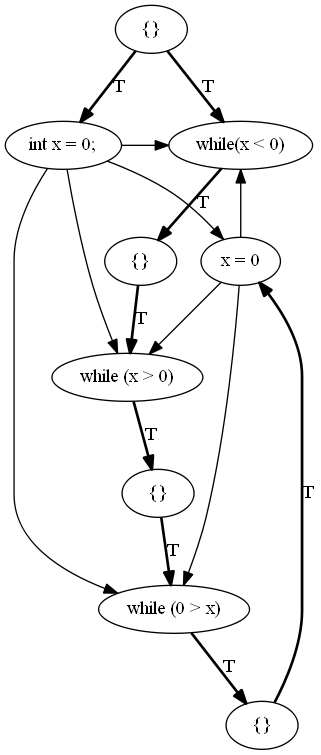
\includegraphics[width=0.8\textwidth]{while_while_while.png}
\end{minipage}
\clearpage


It can be seen from the example that in all the \texttt{while} loops, the variable $x$ is being assigned a new value, and that means that it should have a backedge to every loop which uses $x$. Also, the initial definition of $x$ on line 2 should have an edge to all uses of $x$ too, and the definition of it on line 6.

After addressing the need for the loop references there is another type of statement which is need to be tracked along recursive calls: the Branches. For understanding this, we must take a look at the following code on the left and it's CFG on the right:

\begin{minipage}[c]{0.5\textwidth}
\begin{lstlisting}
int fn(int y){
  int x = 0;
  if (y == 1)
    x = 0;
  else
    x = 1;
  y = x;
}
\end{lstlisting}
\end{minipage}%
\begin{minipage}[c]{0.5\textwidth}
\centering
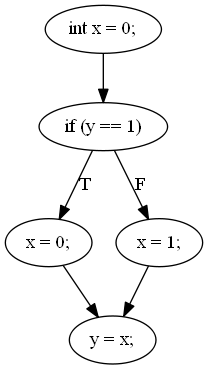
\includegraphics[width=0.6\textwidth]{if_test_cfg.png}
\end{minipage}

From this simple example it can be seen that the value of $y$ on line 7 depends on that which branch gets executed. Therefore we need to draw def-order dependence edges from line 2 to both of the definitions of $x$ under the branch, and also need to draw def-use dependence edges from them to line 7.

This is multiple definition propagation is handled by implementing the set of defs as a multivalue map which has a key which stores the reference to the Clang AST node of the variable declaration (the reference to the \textit{VarDecl}), and a value which is a set which stores the latest definitions of that variable. The value has a single definition in it when outside of a branch, and only stores as many definitions as many branches a branch has, plus optionally the inherited definition before the branch. To distinguish between the definitions, I have used a three valued enum for labeling edges, which have an additional \texttt{None} type among \texttt{True} and \texttt{False}, which represents definitions originated from a parent caller. Originally, the \texttt{None} label is not used in the PDG, only in the algorithm. When it is going into a recursive call, the \texttt{DataEdges} function turns all inherited definitions' edges in \texttt{defs} to \texttt{None}. Since the structure of \texttt{defs} lives only in the algorithm, the original labels of the edges between nodes are not modified. 

In case of an If statement, this amount is two plus one at maximum, but in case of a Switch-Case statement, it could equal to the amount of cases in it plus one. 

To get a picture of what goes on, take a look at the PDG of the example in figure \ref{fig:if_test}. 

\begin{figure}[h]
\centering
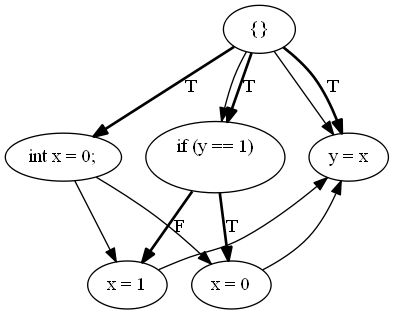
\includegraphics[width=0.6\textwidth]{if_test}
\caption{PDG of example}
\label{fig:if_test}
\end{figure}
When the algorithm visits the \texttt{if} statement, it inherits the initial definition of $x$, and while drawing data dependence edges to both of the branches, it collects their definitions, and returns them to the uppermost Compound statement, which is the root node in this example. Thus when it visits the final node, \texttt{y = x;}, it will know that there has been definitions of $x$ on both branches, so it draws those dependence edges. The algorithm recognize that $x$ is defined on both branches, thus it does not draw dependence edge from the initial definition to \texttt{y = x;}, because the definitions in the branch \textit{intervenes} the path between them, therefore it is not directly dependent on that. But otherwise, if there has been a definition of $x$ in only one of the branches, it would also draw edge over the \texttt{if} statement, between them, because then there would be a path in the CFG which ensure the direct def-use dependence. 
%
The most difficult part of the algorithm to implement was drawing loop-carried dependences. For explaining the details, I must bring up the code example from chapter 2. So, taken that we have the following code:
\clearpage
\begin{lstlisting}
int main(){
  int x = 0;
  int y = 1;
  while(x >= 0){
    if (x > 0){
      y = x; //2. use here 
    }else{
      x = 3;
    }
    x = 2; //1. define here
  }
}
\end{lstlisting}

In this, I have combined a Loop with a Branch to show how would the algorithm determine the loop-carried dependence between line 10. and 6. At the first level of recursion, it visits the only child of the Loop node, a Compound. Then it visits that node's children, the Branch and an Assignment, collecting definitions from them. When the recursion returns to the level of the Loop, the \texttt{defs} set stores the following definitions:

\lstset{numbers=none}
\begin{lstlisting}
[(x,((2,None),(8,False),(10,True))),(y,((3,None),(6,True)))]
\end{lstlisting}

In the set, I have referenced the statements by their line numbers. Each of them has an associated label, which are their relative control dependence label which they are reachable by from their direct parent node. The \texttt{defs} set contains three definitions for variable $x$ and two for $y$, one for each coming from an upper node. The trick is here is in line 9. of the algorithm: in case of visiting a Loop, it visits all it's children again.

Before iterating over them again, it deletes the local definitions, like \texttt{int var = def;}, as those lifetime ends with the scope, and they are created again in every loop iteration. This is also done when returning from a recursive call, to ensure that the algorithm does not carry any `dead` variable. So when it visits the children of the Loop the second time, and starts determining the dependences of statement on line 6, it has the definition of $x$ from line 10 in the \texttt{defs} structure, therefore it will draw an edge between them. It also has the definition of $x$ from line 8, but since their edge labels are not the same, and not a previous parent definition either, there will not be an edge drawn between them. This is handled by deleting the definitions coming from the \textit{then} branch when visiting \textit{else}. 

There is also a fine example of the loop-independent data dependence in the example between statements on line 3. and 6.

The def-use edges are handled on the lines 25-26 in the algorithm. They are much simpler to detect than the def-def edges.

Also, the algorithm handles all combinations of nested control statements, and also the scopes created by Compounds in C++. To demonstrate this, I have created the following code:
\lstset{numbers=left}
\begin{lstlisting}
int f(int x,int y){
  x = 1;
  {
    int x = 2;
    y = x; 
  }
  y = x;
  {
    int x = 3;
    {
      int x = 4;
    }
    x = y;
  }
  return x;
}
\end{lstlisting}

It contains blocks without control structures. I have put the liveness of the variables to the test. As it is known in C++, when a variable with the same name gets declared in an inner scope as the outer scope, the inner one hides the definition of the outer. Luckily, these distictions are handled by Clang, so the algorithm just had to be cared about the inner variables' lifetime. And because the PDG includes these scopes into it's structure with the Compound statements, this is taken care of.
I have included the result PDG here:
\begin{figure}[h]
\centering
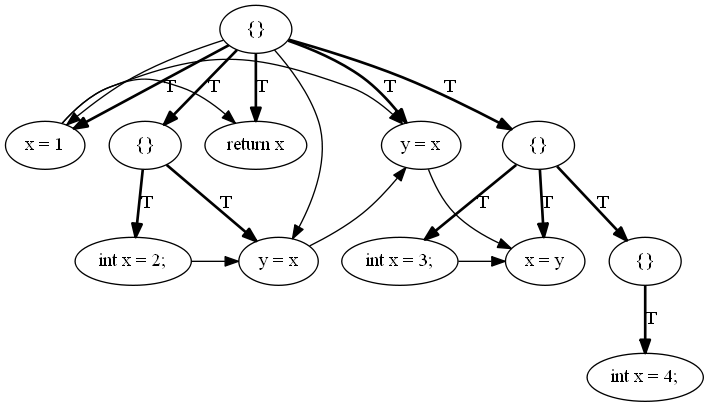
\includegraphics[width=.8\textwidth]{compound_block_test}
\caption{PDG of the scope test}
\label{fig:scope_test}
\end{figure}

In the PDG, it can be seen that the liveness of the definition of $x$ lives out the first inner scope, and also influences the definition of $y$ at line 7.

To note, data dependence analysis would have been simpler if the algorithm used a control-flow graph as input instead of the control-dependence graph. The problems with that that although Clang has an internal CFG module for analysing code, going through that would needed mapping between AST and CFG nodes, and it would added additional cost to the processing of the AST. In this way, the algorithm abstracts itself away from the AST, and this separation enables us to freely extend the algorithm to different kind of language elements of C++.

\section{Implementing slicing}

With having the PDG built up from the source code, the algorithm of slicing gets easier. 



\subsection{Limitations}

%larger ones
%jumps
\begin{lstlisting}[language=C++]
while(x < 0){
  if(y < 2) goto label; 
  x = 2;
}
label:
x = 1;
\end{lstlisting}

In this example, the third line is control dependent on the second, so if we're considering a slice regarding variable $x$ in the last statement, then the second line must be in the slice.

%pointers


\section{Summary and further works}




\addcontentsline{toc}{chapter}{Glossary}
\begin{thebibliography}{Textttext}
\bibitem{weiser84}
  M. Weiser,
  \emph{Program slicing},
  IEEE Transactions on Software Engineering,
  10(4):352-357,
  1984.

\bibitem{slicing-survey}
  Tip, Frank,
  \emph{A survey of program slicing techniques},
  Journal of programming languages 3.3,
  121-189,
  1995. 

\bibitem{horwitz-interproc}
  Horwitz, Susan, Thomas Reps, and David Binkley,
  \emph{Interprocedural slicing using dependence graphs}, 
  ACM Transactions on Programming Languages and Systems,
  (TOPLAS) 12.1: 26-60,
  1990.

\bibitem{information-flow}
  Bergeretti, Jean-Francois, and Bernard A. Carré,
  \emph{Information-flow and data-flow analysis of while-programs},
  ACM Transactions on Programming Languages and Systems,
  (TOPLAS) 7.1: 37-61,
  1985.

\bibitem{use-of-slicing-horwitz}
  Horwitz, Susan, and Thomas Reps,
  \emph{The use of program dependence graphs in software engineering},
  Proceedings of the 14th international conference on Software engineering. 
  ACM,
  1992.

\bibitem{program-analysis-via-graph-reachability-reps}
  Reps, Thomas,
  \emph{Program analysis via graph reachability},
  Information and software technology,
  40.11: 701-726,
  1998.

\bibitem{efficient-pdg}
  Harrold, Mary Jean, Brian Malloy, and Gregg Rothermel,
  \emph{Efficient construction of program dependence graphs},
  ACM SIGSOFT Software Engineering Notes,
  Vol. 18. No. 3. ACM,
  1993.

\bibitem{slicing-oop}
  Larsen, Loren, and Mary Jean Harrold,
  \emph{Slicing object-oriented software},
  Software Engineering,
  Proceedings of the 18th International Conference on. IEEE,
  1996.

\bibitem{slicing-with-jumps}
  Agrawal, Hiralal,
  \emph{On slicing programs with jump statements},
  ACM Sigplan Notices,
  Vol. 29. No. 6. ACM,
  1994.

\bibitem{ottenstein}
  Ottenstein, Karl J., and Linda M. Ottenstein,
  \emph{The program dependence graph in a software development environment},
  ACM Sigplan Notices,
  Vol. 19. No. 5. ACM,
  1984.
  
\bibitem{clang-static-analyzer}
  \emph{Clang Static Analyzer}
  \url{http://clang-analyzer.llvm.org/}

\bibitem{ASTMatchers-reference}
  \emph{AST Matcher Reference}
  \url{http://clang.llvm.org/docs/LibASTMatchersReference.html}
  
\bibitem{Clang-AST}
  \emph{Introduction to the Clang AST}
  \url{http://clang.llvm.org/docs/IntroductionToTheClangAST.html}
  
\bibitem{Wisconsin-slicing-tool}
  \emph{The Wisconsin Program-Slicing Tool}
  \url{http://research.cs.wisc.edu/wpis/slicing_tool/}

\bibitem{Frama-C-slicing}
  \emph{Slicing plug-in for Frama-C}
  \url{https://frama-c.com/slicing.html}

\end{thebibliography}

\end{document}